\documentclass[a4paper,12pt]{scrartcl}
\usepackage{algpseudocode}
\usepackage{inconsolata}
\usepackage{hyperref}
\usepackage{tikz}
\usepackage{listings}
\usepackage{color}
\usepackage{hhline}
\usepackage[T1]{fontenc} 
\usepackage[utf8]{inputenc}
\usepackage{helvet}
\usepackage{listings}
%\usepackage[margin=0.5in]{geometry}
\usepackage{xcolor}
\usepackage{tabularx}
\usepackage{multicol}
\usepackage{amsmath,amssymb,amsthm} 
\usepackage{mathtools}
\usepackage{setspace}

% Tikz settings optimized for causal graphs.
% Just copy-paste this part
\usetikzlibrary{shapes,decorations,arrows,calc,arrows.meta,fit,positioning}
\tikzset{
    -Latex,auto,node distance =1 cm and 1 cm,semithick,
    state/.style ={ellipse, draw, minimum width = 0.7 cm},
    point/.style = {circle, draw, inner sep=0.04cm,fill,node contents={}},
    bidirected/.style={Latex-Latex,dashed},
    el/.style = {inner sep=2pt, align=left, sloped}
}

\onehalfspacing
\newtheorem{theorem}{Theorem}

\lstset{
  basicstyle=\scriptsize\ttfamily,
}

\begin{document}

\newcounter{ctra}
\newcommand{\city}[3]{\setcounter{ctra}{#2}\addtocounter{ctra}{#3}#1[\the\value{ctra}=#2+#3]}
\newcommand{\extracity}[3]{\textbf{\city{#1}{#2}{#3}}}


\section*{Question 1}
\subsection*{Part (a)}
The specification consists of the following parts:
\begin{itemize}
    \item The states consist of elements of the set $S = \{(x, y, z, t, s) \in \{0, 1, 2, 3\}^4 \times \{ left, right \}: x + y = z + t = 3, x \geq z \lor x = 0, y \geq t \lor y = 0\}$, where a 5-tuple $(x, y, z, t, s)$ represents that:
\begin{itemize}
\item there are $x$ missionaries on the left bank.
\item there are $y$ missionaries on the right bank.
\item there are $z$ cannibals on the left bank.
\item there are $t$ cannibals on the right bank.
\item the boat is on side $s$ of the river.
\end{itemize}
\item The initial state is $(3, 0, 3, 0, left)$.
\item Each action is a pair $(a, b)$, $0 < a+b \leq 2 \land (a \geq b \lor a = 0)$, that represents that we load $a$ missionaries and $b$ cannibals into the boat before moving it from one side to the other.
\item $Result((x, y, z, t, left), (a, b)) \coloneqq (x - a, y + a, z - b, t + b, right)$
\item $Result((x, y, z, t, right), (a, b)) \coloneqq (x + a, y - a, z + b, t - b, left)$
\item For each state $s$, $Actions(s) = \{ (a, b) \in \{0, 1, 2\}^2 : 0 < a + b \leq 2, a \geq b \lor a = 0, Result(s, (a, b)) \text{ is a valid state}\}$.
\item A state $(x, y, z, t, direction)$ is a goal if and only if $x = z = 0$.
\item The cost of a path is equal to its length.
\end{itemize}
To estimate the size of the state space, first note that the size of $S$ is bounded above by the size of $\{0, 1, 2, 3\}^4 \times \{left, right\}$, that is, $4^4 \times 2 = 512$. However, by noting that, for a state $(x, y, z, t, s)$, if we fix $x, z, s$ then $y, t$ are also decided (as $y = 3-x, t = 3-z$), and that $x, z$ can be chosen from $\{0, 1, 2, 3 \}$, and $s$ from $\{left, right\}$, we can see that there are at most $4 \times 4 \times 2 = 32$ valid states. This number is very small, and thus by simply bounding the state space size by $32$ we have found a very close estimation for the size of the state space.

\subsection*{Part (b)}
Since the state space is at most $32$, and since all our action costs are equal, a graph search algorithm such as graph breadth-first search would be most appropriate. I wrote a C++ program that implements this algorithm, and included the answer it found below. \\
To see whether graph or tree search is better, first note that each after applying some arbitrary action, there always exists another applicable action that takes us to the state we just left from (i.e. moving the boat back with to the side it came from without changing it's occupants). This implies that tree search will revisit a state on every expansion of a non-root node. This makes tree search much worse than graph search, which will be able to avoid revisiting these states. \\
The solution my program found: \\

\lstinputlisting{sheet1_q1.out}

\section*{Question 2}
\subsection*{Part (a)}
Consider the following system: a robotic arm is trying to build a tower out of wooden blocks of equal size and equal cost. Initially no blocks are placed. At each step, a single action is possible: adding a new block to the top of the tower. Suppose the goal is to build a tower $n$ blocks high. Depth-first search will be able to find the solution in $O(n)$ time, since it will simply continually choose to add a new block to the top of the tower. On the other hand, iterative deepening will find the solution in $O(n^2)$ time, since it must first check whether it can build the tower in $1$ step (which can be checked in $1$ operation), then in $2$ steps (which can be checked in $2$ operations), and so on until it checks whether the tower can be built in $n$ steps, leading to quadratic complexity overall.

\subsection*{Part (b)}
Consider the following system: a robotic arm is trying to build a tower out of wooden blocks of differing sizes and costs. Initially no blocks are placed. The blocks can either have height 1 or height 2. A block of height 2 costs 10 dollars, and a block of height 1 costs 1 dollar. We wish to find the minimal cost to build a tower of height 2. Now, iterative deepening will terminate upon seeing the sole solution whose node is at depth 1 in our search tree (the solution that uses a single block of height 2) ; however, this is suboptimal, as this solution uses 10 dollars, whereas the solution that stacks two blocks of height 1 uses 2 dollars.

\section*{Queston 3}
\subsection*{Part (a)}
I have bolded the entries I filled in:
\begin{itemize}
    \item \city{L}{0}{244}
    \item \extracity{M}{70}{241}, \extracity{T}{111}{329}
    \item \extracity{L}{140}{244}, \extracity{D}{145}{242}, \extracity{T}{111}{329}
    \item \extracity{D}{145}{242}, \extracity{T}{111}{329}, \city{M}{210}{241}, \city{T}{251}{329}
    \item \city{C}{265}{160}, \city{T}{111}{329}, \city{M}{210}{241}, \city{M}{220}{241}, \city{T}{251}{329}
    \item \city{T}{111}{329}, \city{M}{210}{241}, \city{M}{220}{241}, \city{P}{403}{100}, \city{T}{251}{329}, \city{R}{411}{193}, \city{D}{385}{242}
    \item \city{M}{210}{241}, \city{M}{220}{241}, \city{L}{222}{244}, \city{P}{403}{100}, \city{T}{251}{329}, \city{A}{229}{366}, \city{R}{411}{193}, \city{D}{385}{242}
    \item \city{M}{220}{241}, \city{L}{222}{244}, \city{P}{403}{100}, \city{L}{280}{244}, \city{D}{285}{242}, \city{T}{251}{329}, \city{A}{229}{366}, \city{R}{411}{193}, \city{D}{385}{242}
    \item \city{L}{222}{244}, \city{P}{403}{100}, \city{L}{280}{244}, \city{D}{285}{242}, \city{L}{290}{244}, \city{D}{295}{242}, \city{T}{251}{329}, \city{A}{229}{366}, \city{R}{411}{193}, \city{D}{385}{242}
    \item \city{P}{403}{100}, \city{L}{280}{244}, \city{D}{285}{242}, \city{M}{292}{241}, \city{L}{290}{244}, \city{D}{295}{242}, \city{T}{251}{329}, \city{A}{229}{366}, \city{R}{411}{193}, \city{D}{385}{242}, \city{T}{333}{329}
    \item \extracity{B}{504}{0}, \city{L}{280}{244}, \city{D}{285}{242}, \city{M}{292}{241}, \city{L}{290}{244}, \city{D}{295}{242}, \city{T}{251}{329}, \city{A}{229}{366}, \city{R}{411}{193}, \city{D}{385}{242}, \city{T}{333}{329}, \extracity{R}{500}{193}, \extracity{C}{541}{160}
\end{itemize}

The path returned by this is defined by the following sequence of cities:
\begin{center}
Lugoj $\rightarrow$ Mehadia $\rightarrow$ Drobeta $\rightarrow$ Craiova $\rightarrow$ Pitesti $\rightarrow$ Bucharest
\end{center}
Since the straight-line heuristic is admissible, this path must be of optimal length.
\subsection*{Part (b)}
Not necessarily, but since the heuristic we chose is consistent, the path returned will certainly be of the same minimal length -- as it happens, the paths do coincide. On the other hand, the time and space requirements will be smaller, since we never revisit nodes. This is particularly relevant in this case, since every edge in our state graph is bidirectional, and thus when doing tree search we always revisit at least one previously-visited state after any non-root node expansion. Because of this property, not revisiting previously visited states more than makes up for the overhead that graph search incurs by storing previously visited states.

\section*{Question 4}
\subsection*{Part (a)}
\begin{theorem}
    Any consistent heuristic $h$ for which $h(n) \geq 0$ for all nodes $n$, and all goal nodes $n'$ satisfy $h(n') = 0$, is also admissible.
\end{theorem}
\begin{proof}
    I show that, for all nodes $n$, $h(n) \leq h^*(n)$. Since, by assumption, $h(n) \geq 0$ for all nodes $n$, this is sufficient to show admisibility. For some arbitrary $n$, there are two cases:
    \begin{itemize}
        \item If no path from $n$ to some goal node $n'$ exists, then $h^*(n) = \infty$, and so $h(n) \leq h^*(n)$ is immediate.
        \item Otherwise, consider the shortest path from $n$ to any goal node $n'$: $n = n_1, a_1, n_2, a_2, ..., a_{n-1}, n_k = n'$. Now notice that, as $h$ is consistent: \[h(n_i) \leq c(n_i, a_i, n_{i+1}) + h(n_{i+1})\] for $i = 1,...,k-1$. Add all of these together to get: \[\sum_{i=1}^{k-1} h(n_i) \leq \sum_{i=1}^{k-1} c(n_i, a_i, n_{i+1}) + \sum_{i=2}^{k} h(n_i)\] Rearrange to get: \[\sum_{i=1}^{k-1} h(n_i) - \sum_{i=2}^{k} h(n_i) \leq \sum_{i=1}^{k-1} c(n_i, a_i, n_{i+1})\] Since most of the terms in the left hand side cancel, this implies that \[h(n_1) - h(n_k) \leq \sum_{i=1}^{k-1} c(n_i, a_i, n_{i+1})\] Now, since $n = n_1$, $n_k = n'$, and $h(n') = 0$, as $n'$ is a goal node: \[h(n) \leq \sum_{i=1}^{k-1} c(n_i, a_i, n_{i+1})\] And, since $n_1, a_1, n_2, a_2, ..., n_{k-1}, n_k$ is the shortest path from $n$ to any goal node, we have that the right hand side of this equation is $h^*(n)$. So $h(n) \leq h^*(n)$, as required.
    \end{itemize}
\end{proof}

\subsection*{Part (b)}
The described graph: \\

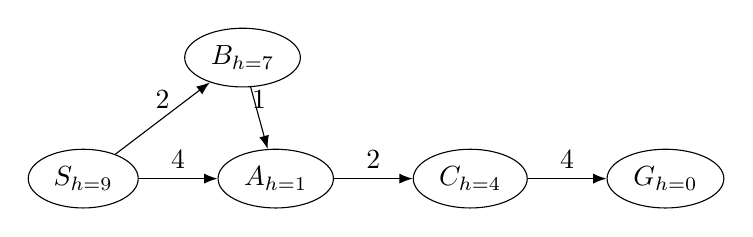
\begin{tikzpicture}
    \node[state] (1) {$S_{h=9}$};
    \node[state] (2) [right =of 1] {$A_{h=1}$};
    \node[state] (3) [above right =of 1] {$B_{h=7}$};
    \node[state] (4) [right =of 2] {$C_{h=4}$};
    \node[state] (5) [right =of 4] {$G_{h=0}$};

    \path (1) edge node[above] {$4$} (2);
    \path (1) edge node[above] {$2$} (3);
    \path (3) edge node[above] {$1$} (2);
    \path (2) edge node[above] {$2$} (4);
    \path (4) edge node[above] {$4$} (5);
\end{tikzpicture}

This heuristic is indeed admissible (since $h^*(G) = 0 \geq 0 = h(G), h^*(C) = 4 \geq 4 = h(C), h^*(A) = 6 \geq 1 = h(A), h^*(B) = 7 \geq 7 = h(B), h^*(S) = 9 \geq 9 = h(S)$, and also since all heuristic values are non-negative). However, the heuristic is not consistent, as: $h(B) = 7 > 2 = 1 + 1 = h(A) + cost(B, A)$.

\subsection*{Part (c)}
To illustrate the working of $A^*$ graph search, I will list the nodes that are expanded, in order, together with the nodes in the priority-queue of nodes to be visited, in increasing order of $f = g+h$, using the same format for nodes' $f$, $g$ and $h$ values as in problem 2:

\begin{tabular}{|l|l|}
\hline
    Currently expanded node & Nodes in priority-queue \\
\hline
    $S[9=0+9]$ & $A[5 = 4+1], B[9 = 2 + 7]$ \\
\hline
    $A[5=4+1]$ & $B[9 = 2 + 7], C[10=6+4]$ \\
\hline
    $B[9=2+7]$ & $C[10=6+4]$ \\
\hline
    $C[10=6+4]$ & $G[10=10+0]$ \\
\hline
    $G[10=10+0]$ & \\
\hline
\end{tabular}

So $A^*$ graph search finds a path of length $10$ from $S$ to $G$: $S \rightarrow A \rightarrow C \rightarrow G$. This is not optimal, as there exists a path of length 9: $S \rightarrow B \rightarrow A \rightarrow C \rightarrow G$.

\section*{Question 5}
\begin{theorem}
    If all paths in a search graph are nondecreasing in terms of $f$ values, then the heuristic $h$ that we used is consistent.
\end{theorem}
\begin{proof}
    To show this, I show that for any directed edge from node $A$ to node $B$ from our search graph, realised by some action $a$, we have that $h(A) \leq h(B) + c(A, a, B)$. \\
    Consider any such $A$, $B$, $a$ in the graph. Since all paths are nondecreasing in terms of $f$ values, by considering the path that consists only of the nodes $A$ and $B$, we get that $f(A) \leq f(B)$. This implies, by definition of $f$, that $g(A) + h(A) \leq g(B) + h(B)$. Now, note that, by definition of $g$, $g(B) \leq g(A) + c(A, a, B)$, since if some path of length $g(A)$ exists from the initial state to $A$, then one of length $g(A) + c(A, a, B)$ also must exist to node $B$, and thus $g(B)$ cannot exceed this value. Substituting this into the first equation, we get that $g(A) + h(A) \leq g(B) + h(B) \leq g(A) + c(A, a, B) + h(B)$. Subtracting $g(A)$, we get that $h(A) \leq h(B) + c(A, a, B)$, as required.
\end{proof}

\section*{Question 6}

\subsection*{Part (a)}
\textit{(Note: I consider only those tours that begin and end with some arbitrary distinguished vertex $v_s$. The choice of this vertex does not matter, as any tour that begins and ends with this vertex can easily be transformed to generate ones that begin and end with any vertex. I do this both for efficiency, as this reduces the number of states I visit by a factor of $|V|$, and for simplicity).} \\
The core idea of my formalisation is that each path in the graph is though of as a state, and the act of extending such a path by one vertex is though of as an action. Only valid tours will be accepted as goal states. In order to make this more efficient, rather than allowing all possible actions, I only allow those that do not make it impossible to eventually reach a tour (i.e. in all reachable states I try to make the first $|V|$ vertices distinct, and I try to make the $|V|+1^{th}$ vertex equal the first one). A formal description of this idea follows:
\begin{itemize}
    \item The states are taken from the set of possible paths through the graph i.e.:
        \[
            \textsc{States} \coloneqq \{ \langle v_1, ..., v_k \rangle : \forall i \in \{1, ..., k-1 \} . \langle v_i, v_{i+1} \rangle \in E \}
        \]
    \item The start state is the path $\langle v_s \rangle$.
    \item An action shall consist of a single vertex $v \in V$.
    \item For each state $s = \langle v_1, ..., v_k\rangle$ and each action $v \in \textsc{Actions(s)}$, the result of applying $v$ to $s$ is a path that begins with the path $s$, but with the vertex $v$ appended i.e.:

        \[
            \textsc{Result}(s, v) \coloneqq \langle v_1, ..., v_k, v \rangle
        \]
    \item For some state $s = \langle v_1, ..., v_k \rangle$, the set of available actions is the set of vertices $v$ for which there exists an edge from $v_k$ to $v$, and for which either $k < |V|$ and $v$ does not appear among $v_1, ..., v_k$, or $k = |V|$ and $v = v_1$ i.e.:
        \[
            \textsc{Actions}(s) \coloneqq \{ v \in V : \langle v_k, v \rangle \in E \land ((k < |V| \land v \neq v_1 \land ... \land v \neq v_k) \lor (k = |V| \land v = v_1)) \}
        \]
    \item For each pair of states $(x, y)$, and action $a$ taking $x$ to $y$, the step cost of this action is equal to the weight of the last edge in path $y$, i.e.:
        \[
            c(x, a, y) \coloneqq w(\langle p, q \rangle)
        \]
        where $y = \langle v_1, ..., p, q \rangle$ Equivalently, this could have been defined as the length of the edge that begins at the last vertex of $x$, and ends at $a$.
    \item A state $s = \langle v_1, ..., v_k \rangle$ is a goal state if and only if the path it represents is a tour.
    \item The state space is the set of states that we can reach from the initial state. Due to the way in which I defined \textsc{Actions} and the initial state, the only states I can possibly reach from the initial state are either tours, or paths of at most $|V|$ distinct vertices, either of which must begin with $v_s$, viz.:
    \[
        \{ \langle v_1, ..., v_k \rangle : v_1 = v_s \land ((k \leq |V| \land v_1, ..., v_k \text{ distinct}) \lor (k = |V|+1 \land \langle v_1, ..., v_k \rangle \text{ is a tour})) \}
    \]
\end{itemize}

This formalisation can only ever accept as goals states that represent tours. Moreover, it is easy to see that any state that represents a tour (that begins and ends with $v_s$) can be reached from the initial state -- as any tour of the form $\langle v_1, v_2, ..., v_n, v_1 \rangle$ where $v_1 = v_s$ can be reached by succesively applying actions $v_2, v_3, ..., v_n, v_1$ to initial state $\langle v_1 \rangle$. This implies that the formalisation is faithful to the initial problem, as all goal states that we can reach represent actual solutions for the initial problem, and as we can potentially reach any such solution.

\subsection*{Part (b)}
Take $g$ to be the path cost function that results from using the step cost defined in Part (a) (i.e. I consider the path cost to be the sum of the set costs of all the actions taken during the path). \\
To see why uniform-cost search equipped with this cost function will certainly find a optimal tour consider any path of states $p = s_1, a_1, ..., s_n, a_n, s_{n+1}$, where $s_1$ is the initial state $\langle v_s \rangle$, and where node $n$ corresponds to state $s_{n+1}$ in this path. Here, the path cost of $n$ will be, by definition, equal to:
\[
    g(n) = \sum_{i=1}^n c(s_i, a_i, s_{i+1})
\]
Now, note that, by definition of $Result$, each path of vertices $s_i$ has length one less than the following path of vertices $s_{i+1}$, and moreover, $s_i$ is a prefix of $s_{i+1}$. This, together with the fact that $s_1$ is a path of length one, implies, through induction, that, for some $v_1, ..., v_{n+1}$, we have that $s_i = \langle v_1, ..., v_i \rangle$ for $i = 1, 2, ..., n+1$, and thus that the last edge of $s_{i+1}$ is $\langle v_i, v_{i+1} \rangle$. This implies, by definition of $c$, that $c(s_i, a_i, s_{i+1}) = w(\langle v_i, v_{i+1} \rangle)$. Substituting this into the previous equation, we get:
\[
    g(n) = \sum_{i=1}^n w(\langle v_i, v_{i+1} \rangle)
\]
Note that the right hand side of this is equal to $w(p)$ overall, so $g(n) = w(p)$. Now this implies that if we find a goal node (i.e. one whose state corresponds to a tour, as shown in the previous part) of minimal path cost, then we will thus find the tour of minimal weight i.e. an optimal tour. Uniform-cost search will certainly find such a node, since all step costs are positive and not less than $\epsilon = \min_{\langle a, b \rangle \in E} w(\langle a, b \rangle)$, where $\epsilon > 0$; and in such conditions, uniform-cost search is complete\\
Uniform cost search may be very inefficient with such a path cost though, since the path cost $C^*$ of an optimal solution may be very large compared to the minimal step cost $\epsilon$; indeed, it may be the case that $C^* = |V| * \epsilon$, if the optimal tour consists of $|V|$ edges of length $\epsilon$. In such cases, the work needed by uniform-cost search is bounded by $O(b^{|V|})$. Since $b$ can be even on the order of $|V|$, this is very large.

\subsection*{Part (c)}
The exact heuristic $h^*(n)$ where $n$ corresponds to a state $s$ with $s = \langle v_1, ..., v_k \rangle$ tells us the minimal total cost of a sequence of edges that need to be added to the end of the path $s$ in order to make it become a tour. This can be expressed formally by:
\[
    h^*(n) \coloneqq
    \begin{dcases}
        \infty \text{, if no path from $n$ to a goal node exists} \\
        \min \{ w(\langle v_1, ..., v_{|V|+1} \rangle) : v_{k+1}, ..., v_{|V|+1} \in V, \langle v_1, ..., v_{|V|+1} \rangle \text{ is a tour} \} - w(s) \text{, otherwise}
    \end{dcases}
\]
For any exact heuristic (including the one discussed here), assuming that at least one path from the initial node to a goal node exists, A* tree search will always explore only those nodes that are on at least one optimal path from the start node to some goal node. The reason is that the fitness function $f(n) = g(n) + h^*(n)$ tells us the length of the shortest path between the initial node and any goal node that also passes through $n$ (since $g(n)$ tells us the cost of the part of this path that is between the initial node and $n$, and $h^*(n)$ will tell us the cost of the part of this path that is between $n$ and a goal node). Since those nodes which are on at least one optimal path minimise this value, and $A^*$ will (if there exists at least one path to a goal node) always have one such node to explore, this implies that $A^*$ can only ever explore those nodes that are on at least one optimal path to a goal. \\
(This is not necessarily very efficient, though, in the case where there are very many optimal paths. Imagine a search tree that looks like a binary tree of some depth $d$, where all the step costs are 1, with every single node at depth $d$ being a goal node. In such a tree, all nodes have equal fitness value, since $g(n)$ will equal the depth of $n$, and $h^*(n)$ will equal $d$ minus this depth, and so $f(n) = d$. Thus, in such a case, the search will nondeterministically explore the tree until it reaches a result. It could thus explore all $2^d$ nodes, rather than directly going to a goal in $O(d)$). \\
Such a heuristic cannot be used to solve search problems, since computing it is tantamount to solving the problem itself.

\subsection*{Part (d)}
Let $\mathcal{F}(V, E)$ be the set of spanning forests of the graph defined by vertex set $V$ and edge set $E$. Write $e \in F$ for some edge $e$ and forest $F$ if and only if the edge $e$ appears in $F$. Also, let $w(F)$ be the sum of the weights of the edges in some forest $F$. Now, for any node $n$ that holds state $s = \langle v_1, ..., v_k \rangle$, let $h(n)$ be defined by:
\[
    h(n) \coloneqq
    \begin{cases}
        0 & \text{, $n$ is a goal node} \\
        \min \{ w(F) : F \in \mathcal{F}(V, E) \land \langle v_1, v_2 \rangle \in F \land ... \land \langle v_{k-1}, v_k \rangle \in F \} - w(s) & \text{, otherwise}
    \end{cases}
\]
That is, if $n$ is a goal node, then $h(n)$ is 0; otherwise, $h(n)$ is the sum of the costs of the edges of the minimal spanning forest of $G$ that contains all the edges of $s$, if we ignore the costs of the edges already present in $s$. \\
Thus, to calculate $h(n)$, where $n$ contains state $s = \langle v_1, ..., v_k \rangle$, in the case where $n$ is not a goal node, we want to find a spanning forest $F$ such that $w(F) - w(s)$ is minimised, subject to the constraint that $F$ contains all the edges in $s$. To do this, consider the following edge cost function:

\[
    w'(e) \coloneqq
    \begin{cases}
        -1 & \text{, if }e = \langle v_1, v_2 \rangle \lor ... \lor e = \langle v_{k-1}, v_k \rangle \\
        w(e) & \text{, otherwise}
    \end{cases}
\]

Note: for any spanning forest $F$ that contains the edges in the path $s$, we can show that $w(F) - w(s) = w'(F) + (k-1)$ (since both of these are simply the total cost w.r.t. $w$ of the edges of $F$ that do not appear in the path $s$). This means that, to minimise $w(F) - w(s)$ subject to the constraint that $F$ contains all edges in path $s$, I can just as well minimise $w'(F) + k - 1$ subject to that same constraint. But now, note that the minimal spanning forest $F$ for $G$ w.r.t. $w'$ will always contain all the edges of path $e$, as these have the smallest costs out of all the edges of the graph. This implies that the global minimum of $w'(F) + k - 1$ (i.e. taking $F$ to be a minimal spanning forest w.r.t. $w'$) also satisfies our constraint. We can thus choose $F$ to be this global minimum:

\begin{algorithmic}[1]
    \Function{$h$}{$n$}
    \If{$n$ is a goal state}
        \State \Return 0
    \EndIf
    \State $s \gets \text{the state of } n$
    \State Construct $w'$ out of $w$ and $s$ as described above.
    \State Find the minimal spanning forest $F$ of $(V, E)$ with respect to cost function $w'$ \footnote{This can be done with any classical MST algorithm, such as Prim's algorithm, Kruskal's algorithm or Borůvka's algorithm}.
    \State \Return $w(F) - w(s)$ 
    \EndFunction
\end{algorithmic}

This heuristic is more suitable for $A^*$ than $h^*$ since it can be computed without needing to solve an instance of the problem we are trying to solve with $A^*$.

\subsection*{Part (e)}
\begin{theorem}
    The $h$ from the previous part is admissible
\end{theorem}
\begin{proof}
    I show this by showing that, for any node $n$ which holds state $s = \langle v_1, ..., v_k \rangle$, it is true that $h(n) \leq h^*(n)$. That $h(n) \geq 0$ is immediate from the fact that $h(n)$ is either 0 or the sum of the costs of some set of edges w.r.t $w$, and these costs are positive. There are two cases:
    \begin{itemize}
        \item If no path exists from $n$ to a goal node, then $h^*(n) = \infty$, and the result is immediate.
        \item If some such path exists, then by definition of $h^*(n)$, $h^*(n) = w(\langle v_1, ..., v_{|V|+1} \rangle) - w(s)$, for some vertices $v_{k+1}, ..., v_{|V|+1} \in V$ for which $\langle v_1, ..., v_{|V|+1} \rangle$ is a tour. Now:
\begin{align*}
    h^*(n) &= w(\langle v_1, ..., v_{|V|+1} \rangle) - w(s) \\
           &= w(\langle v_1, v_2 \rangle) + ... + w(\langle v_{|V|-1}, v_{|V|} \rangle) + w(\langle v_{|V|}, v_{|V|+1} \rangle) - w(s) \tag{by definition of $w$} \\
           &\geq w(\langle v_1, v_2 \rangle) + ... + w(\langle v_{|V|-1}, v_{|V|} \rangle) - w(s) \tag{as $w(\langle v_{|V|}, v_{|V|+1} \rangle) \geq 0$}
\end{align*}
            But, now, note that, as $\langle v_1, ..., v_{|V|+1} \rangle$ is a tour, and thus $v_1, ..., v_{|V|}$ are distinct, and $\langle v_1, v_2 \rangle, ..., \langle v_{|V|-1}, v_{|V|} \rangle \in E$, we have that the subgraph $T_0$ defined by these edges is a spanning forest of our graph that contains all of the edges in the path $\langle v_1, ..., v_{|V|} \rangle$ i.e. $T_0 \in \mathcal{F}(V, E) \land \langle v_1, v_2 \rangle \in T_0 \land ... \land \langle v_{|V|-1}, v_{|V|} \rangle \in T_0$. Thus, $w(T_0)$ is an upper bound for the first term in the second case of the definition of $h$, so:
\begin{align*}
    h^*(n) &\geq w(\langle v_1, v_2 \rangle) + ... + w(\langle v_{|V|-1}, v_{|V|} \rangle) - w(s) \\
           &\geq w(T_0) - w(s) \tag{by definition of $F$} \\
           &\geq \min \{ w(F) : F \in \mathcal{F}(V, E) \land \langle v_1, v_2 \rangle \in F \land ... \land \langle v_{|V|-1}, v_{|V|} \rangle \in F \} - w(s) \tag{as $T_0$ is in the set we take the minimum of here} \\
           &\geq h(n)
\end{align*}
            So in this case as well we have that $h^*(n) \geq h(n)$.
    \end{itemize}
    So overall $h$ is admissible.
\end{proof}


\end{document}
